\documentclass[a4paper, 12pt]{article}
%\usepackage[a4paper]{geometry}  % More space on A4 paper
\usepackage[a4paper, left=2cm, right=2cm, top=2cm, bottom=2cm]{geometry}
\usepackage{graphicx,epstopdf}
\usepackage{dcolumn}
\newcolumntype{d}[1]{D{.}{.}{#1}}
\usepackage{float}
\usepackage{tabularx,ragged2e,booktabs,caption}
\usepackage{array}
\usepackage{multirow}
\usepackage[svgnames]{xcolor}
\usepackage{enumitem}
\usepackage{tikz}
\usepackage[utf8]{inputenc}
\usepackage{forest}
\usepackage{eurosym}
%%%%%%%%%%% mathematics %%%%%%%%%%%%%%%%%%
\usepackage{amsmath,amsfonts,amssymb, amsthm}
\usepackage{mathtools}
\usepackage[noend]{algpseudocode}
\usepackage{algorithm}
\usepackage{titling}
\setlength{\droptitle}{-5em}
\theoremstyle{definition}
\newtheorem{definition}{Definition}[section]
\newtheorem{theorem}{Theorem}
\newcommand\numberthis{\addtocounter{equation}{1}\tag{\theequation}}

% Use the bibliography, with \citet{}, \citep{}
\usepackage{natbib}
\usepackage{hyperref}


%%%%%%%%%%%%%%%%%%%%%%%%%%%% START HERE %%%%%%%%%%%%%%%%%%%%%%%%%%%% 

\title{\Huge Group Assignment I\\[0.5em]\large Advanced Econometrics 2026--2027}
\author{\large Phuc Nguyen (2779150)\\\normalsize Email: t.t.p.nguyen2@student.vu.nl\\[0.3cm]
\large Tu Nguyen (2849240)\\\normalsize Email: x.nguyenanhtu@student.vu.nl\\[0.3cm]
\large Boris de Buck (2732664)\\\normalsize Email: b.m.de.buck@student.vu.nl\\[0.3cm]
\large Anna van Dam (2861128)\\\normalsize Email: a.l.van.dam2@student.vu.nl}
\date{\today}



\begin{document}
\maketitle
\newpage


\section*{Question 1}

First write out $\sigma^2_{t+1}(\sigma_t^2, \epsilon_t)$, i.e. write the volatility equation as a function of the
innovations.

We know:
\[x_t=\mu+\lambda\sigma_t^2+\sigma_t\varepsilon_t
\]

and by the given equation for $\sigma_t$ we know:
\[
\sigma_{t+1}^2=\omega+\Big(\alpha+\delta\tanh(-\gamma x_t)\Big)\left(\frac{x_t-\mu-\lambda\sigma_t^2}{\sigma_t}\right)^2+\beta\sigma_t^2.
\]

Substituting now gives us:
\begin{align*}
\sigma_{t+1}^2&=\omega+\Big(\alpha+\delta\tanh\big(-\gamma(\mu+\lambda\sigma_t^2+\sigma_t\varepsilon_t)\big)\Big)\left(\frac{(\mu+\lambda\sigma_t^2+\sigma_t\varepsilon_t)-\mu-\lambda\sigma_t^2}{\sigma_t}\right)^2+\beta\sigma_t^2 \\[4pt]
&=\omega+\Big(\alpha+\delta\tanh\big(-\gamma(\mu+\lambda\sigma_t^2+\sigma_t\varepsilon_t)\big)\Big)\left(\frac{\sigma_t\varepsilon_t}{\sigma_t}\right)^2+\beta\sigma_t^2 \\[4pt]
&=\omega+\Big(\alpha+\delta\tanh\big(-\gamma(\mu+\lambda\sigma_t^2+\sigma_t\varepsilon_t)\big)\Big)\varepsilon_t^2+\beta\sigma_t^2.
\end{align*}

We have now written $\sigma_{t+1}^2(\sigma_t, \varepsilon_t)=\omega+\Big[\alpha+\delta\tanh\big(-\gamma(\mu+\lambda\sigma_t^2+\sigma_t\varepsilon_t)\big)\Big]\varepsilon_t^2+\beta\sigma_t^2$. We want to show that $\{\sigma_t\}_{t\epsilon Z}$ is SE. We can do this by Bougerol's Theorem.

\bigskip

\noindent \textbf{A1} $\{\varepsilon_t\}_{t\in\mathbb{Z}}$ is SE. This holds since $\{\varepsilon_t\}\sim TID(v)$ is iid and any iid sequence is SE.

\bigskip

\noindent \textbf{A2} There should exist a finite initialization $\sigma_1^2$ such that $\mathbb{E}\big[\log^+|\sigma_2^2(\sigma_1^2,\varepsilon_1)|\big]<\infty$. We have:
\begin{align*}
\mathbb{E}\big[\log^+|\sigma_2^2(\sigma_1^2,\varepsilon_1)|\big]
&= \mathbb{E}\Big[\log^+\Big|\omega+\big[\alpha+\delta\tanh\big(-\gamma(\mu+\lambda\sigma_1^2+\sigma_1\varepsilon_1)\big)\big]\varepsilon_1^2+\beta\sigma_1^2\Big|\Big] \\[4pt]
&\le \mathbb{E}\Big[\Big|\omega+\big[\alpha+\delta\tanh\big(-\gamma(\mu+\lambda\sigma_1^2+\sigma_1\varepsilon_1)\big)\big]\varepsilon_1^2+\beta\sigma_1^2\Big|\Big] && (\log^+|z|\le|z|) \\[4pt]
&\le |\omega| + \mathbb{E}\Big[\big|\alpha+\delta\tanh\big(-\gamma(\mu+\lambda\sigma_1^2+\sigma_1\varepsilon_1)\big)\big|\,\varepsilon_1^2\Big] + |\beta|\,|\sigma_1^2| &&(\text{triangle inequality}) \\[4pt]
&\le |\omega| + \mathbb{E}\Big[\big(|\alpha|+|\delta|\,|\tanh(\cdots)|\big)\varepsilon_1^2\Big] + |\beta|\,|\sigma_1^2| &&(\text{triangle inequality}) \\[4pt]
&\le |\omega| + \mathbb{E}\big[(|\alpha|+|\delta|)\,\varepsilon_1^2\big] + |\beta|\,|\sigma_1^2| &&(-1\le\tanh(\cdot)\le1) \\[4pt]
&= |\omega| + (|\alpha|+|\delta|)\,\mathbb{E}[\varepsilon_1^2] + |\beta|\,|\sigma_1^2| \\[4pt]
&< \infty.
\end{align*}

\par This is finite since $\omega,\alpha,\beta,\delta$ are finite parameters, $\mathbb{E}[\varepsilon_1^2]<\infty$ for $\varepsilon_1\sim TID(v)$ with $v>2$, and $\sigma_1^2$ is a finite initialization. So A2 holds.

\bigskip

\noindent \textbf{A3} The contraction holds when
\[
\mathbb{E}\left[\log\sup_{x\in\mathcal{X}}\left|\frac{\partial\phi(x,\varepsilon_t)}{\partial x}\right|\right]<0.
\]

\par Here $\phi(\sigma_t^2,\varepsilon_t)=\omega+\big[\alpha+\delta\tanh\big(-\gamma(\mu+\lambda\sigma_t^2+\sigma_t\varepsilon_t)\big)\big]\varepsilon_t^2+\beta\sigma_t^2$.
 
\par We recall also that $\dfrac{d\tanh(x)}{dx}=1-\tanh^2(x)$.
 
\par By the chain rule,
\[
\frac{\partial\phi(\sigma_t^2,\varepsilon_t)}{\partial\sigma_t^2}=\delta\varepsilon_t^2\Big(1-\tanh^2\big(-\gamma(\mu+\lambda\sigma_t^2+\sigma_t\varepsilon_t)\big)\Big)\cdot(-\gamma)\left(\lambda+\frac{\varepsilon_t}{2\sqrt{\sigma_t^2}}\right)+\beta.
\]

\par We then bound,
\begin{align*}
\left|\frac{\partial\phi(\sigma_t^2,\varepsilon_t)}{\partial\sigma_t^2}\right|
&\le |\gamma||\delta|\,\varepsilon_t^2\,\Big|1-\tanh^2\big(-\gamma(\mu+\lambda\sigma_t^2+\sigma_t\varepsilon_t)\big)\Big|\left(|\lambda|+\frac{|\varepsilon_t|}{2\sqrt{\sigma_t^2}}\right)+|\beta| &&(\text{triangle inequality}) \\[4pt]
&\le |\gamma||\delta|\,\varepsilon_t^2\left(|\lambda|+\frac{|\varepsilon_t|}{2\sqrt{\sigma_t^2}}\right)+|\beta| &&(0\le1-\tanh^2(\cdot)\le1) \\[4pt]
&\le |\gamma||\delta|\,\varepsilon_t^2\left(|\lambda|+\frac{|\varepsilon_t|}{2\sqrt{\omega}}\right)+|\beta| &&(\sigma_t^2\ge\omega \;\Rightarrow\; \tfrac{1}{2\sqrt{\sigma_t^2}}\le\tfrac{1}{2\sqrt{\omega}}) \\[4pt]
&= |\gamma|\left(|\lambda\delta|\varepsilon_t^2+\frac{|\delta||\varepsilon_t|^3}{2\sqrt{\omega}}\right)+|\beta|,
\end{align*}
\par where $\sigma_t^2\ge\omega$ holds for all $t$ since $\alpha>|\delta|$ and $|\tanh(\cdot)|\le1$, $\alpha+\delta\tanh(-\gamma x_{t-1})\ge\alpha-|\delta|>0$, so the middle term of the $\sigma_t^2$-recursion is non-negative and since $\beta\ge0$ so is $\beta\sigma_{t-1}^2$. Hence $\sigma_t^2\ge\omega$.
 
\par Therefore,
\[
\mathbb{E}\left[\log\sup_{x\in\mathcal{X}}\left|\frac{\partial\phi(x,\varepsilon_t)}{\partial x}\right|\right]\le\mathbb{E}\left[\log\left(|\gamma|\left(|\lambda\delta|\varepsilon_t^2+\frac{|\delta||\varepsilon_t|^3}{2\sqrt{\omega}}\right)+|\beta|\right)\right] < 0,
\]
\par which is exactly the condition given in the question.


\noindent Thus, by Bougerol's theorem, $\{\sigma_t^2\}{t\in\mathbb{Z}}$ converges to a SE process. Since $x_t=\mu+\lambda\sigma_t^2+\sigma_t\varepsilon_t$ is a measurable function of the jointly SE sequence $\{(\sigma_t,\varepsilon_t)\}{t\in\mathbb{Z}}$, in this case $\{x_t\}_{t\in\mathbb{Z}}$ is also SE by Krengel's theorem.









\section*{Question 2}

\begin{figure}[H]
    \centering
    
\includegraphics[width=0.9\textwidth]{fig2.1.png}
    \caption{News impact curves of the GARCH-M-L model for different values of $\delta$ and $\gamma$.}
    \label{fig:fig2.1}
\end{figure}

The news impact expression is given by $\mathrm{NIC}(x_{t-1}) = (\alpha + \delta \tanh(-\gamma x_{t-1})) x_{t-1}^2$.
Looking at \autoref{fig:fig2.1}, it can be seen that different values of $\delta$ and $\gamma$ have a significant impact on the shape of the news impact curve. 
When $\delta > 0$, the news impact curve is asymmetric, indicating that negative shocks have a larger effect on volatility than positive shocks of equal size. And 
$\delta < 0$ mirrors it. When $\delta \rightarrow 0$, all curves collapse to a symmetric one regardless of $\gamma$. Indeed,
as $\delta = 0, \gamma$ is dropped, the expression reduces to $\alpha x_{t-1}^2$, which is a parabola. 

\par Regarding $\gamma$, it controls how abruptly the asymmetry switches on: $\gamma = 0.01$ is almost symmetric since 
$\tanh(x) \approx x$ for relatively small $x$. When $\gamma$ increases, the asymmetry becomes more pronounced. As $\gamma \rightarrow \infty$, the $\tanh$ function approaches a step function, 
giving $\alpha + \delta$ for negative shocks and $\alpha - \delta$ for positive shocks.



\section*{Question 3}

\begin{table}[H]
    \centering
    \caption{Descriptive statistics of the daily holding period returns}
    \begin{tabular}{lrrrr}
        \toprule
        & PFE & JNJ & MRK & AAPL \\
        \midrule
        Number of observations & 3270 & 3270 & 3270 & 3270 \\
        Mean & 0.041 & 0.046 & 0.057 & 0.107 \\
        Median & 0.000 & 0.036 & 0.046 & 0.089 \\
        Standard deviation & 1.368 & 1.076 & 1.306 & 1.783 \\
        Minimum & -7.735 & -10.038 & -9.863 & -12.865 \\
        Maximum & 10.855 & 7.998 & 10.408 & 11.981 \\
        Skewness & 0.223 & -0.150 & 0.083 & -0.076 \\
        Excess kurtosis & 5.294 & 9.370 & 6.637 & 5.360 \\
        \bottomrule
    \end{tabular}
    \label{tab:descrp_stats}
\end{table}


\autoref{tab:descrp_stats} provides descriptive statistics of the daily holding period returns for Pfizer (PFE), 
Johnson \& Johnson (JNJ), Merck \& Co. (MRK), and Apple (AAPL). The number of observations is 3270 for each stock, and 
the mean daily return ranges from 0.041\% for PFE to 0.107\% for AAPL. In terms of volatility, AAPL has the highest standard 
deviation while JNJ has the lowest indicating that AAPL is more volatile compared to the other stocks (e.g. JNJ), which can be observed in \autoref{fig:fig3.1}. The minimum and 
maximum daily returns also vary across the stocks, with AAPL having the largest range of returns, from -12.865\% to 11.981\%,
while JNJ has the smallest range, from -10.038\% to 7.998\%. The skewness and excess kurtosis values indicate that the 
return distributions are not perfectly normal, with some stocks exhibiting left-skewed distributions (JNJ and AAPL) and 
others right-skewed (PFE and MRK). All stocks show excess kurtosis greater than 3, suggesting that the return distributions 
have heavier tails than a normal distribution. 

\begin{figure}[H]
    \centering
    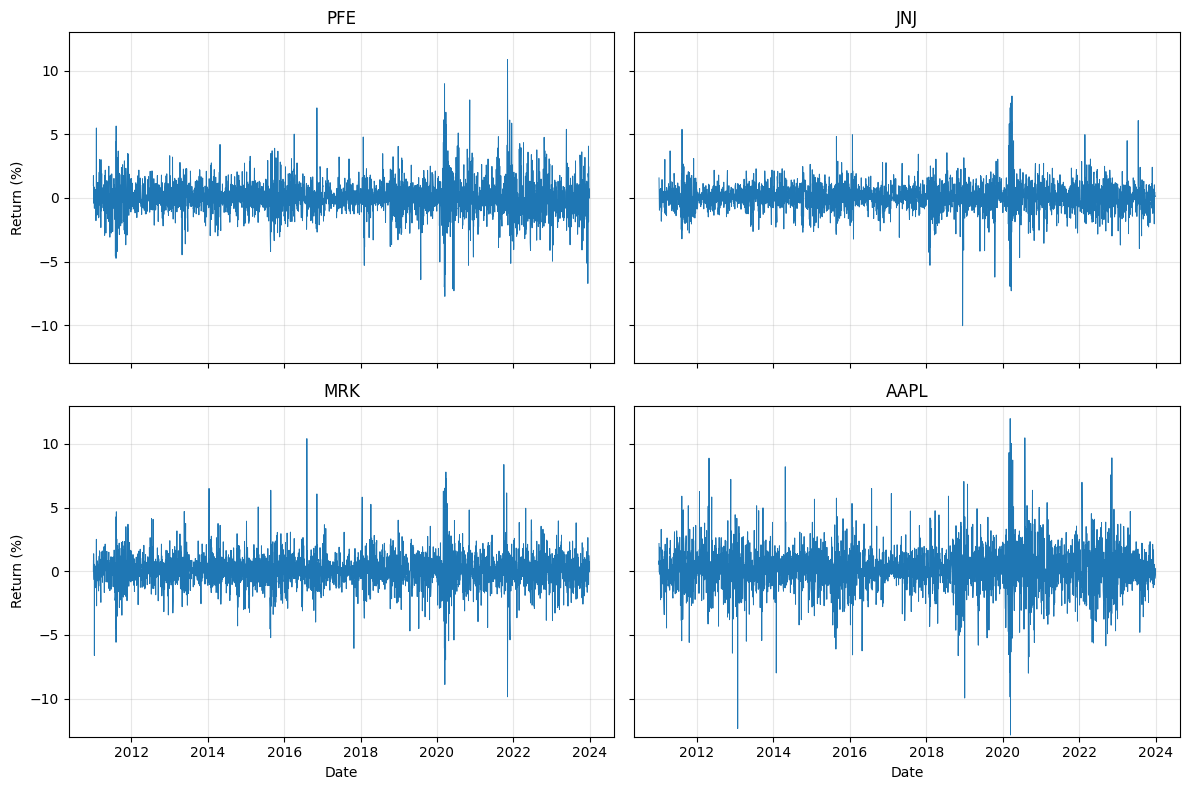
\includegraphics[width=0.9\textwidth]{fig3.1.png}
    \caption{Daily holding period returns of Pfizer, Johnson \& Johnson, Merck \& Co., and Apple.}
    \label{fig:fig3.1}
\end{figure}

It is also remarkable that the returns of all four stocks exhibit volatility clustering, where periods of high volatility are followed by
periods of low volatility and vice versa. Looking at the time around the COVID-19 pandemic, we can see that there is a 
significant fluctuation in volatility for all four stocks, which is consistent with the market-wide uncertainty and turbulence during that period.
\section*{Question 4}

\begin{table}[H]
    \centering
    \caption{Maximum likelihood estimates of the three volatility models}
    \label{tab:q4_estimates}
    \footnotesize
    \setlength{\tabcolsep}{3pt}
    \resizebox{\textwidth}{!}{%
    \begin{tabular}{l rrr rrr rrr}
        \toprule
        & \multicolumn{3}{c}{PFE} & \multicolumn{3}{c}{JNJ} & \multicolumn{3}{c}{MRK} \\
        \cmidrule(lr){2-4} \cmidrule(lr){5-7} \cmidrule(lr){8-10}
        & M1 & M2 & M3 & M1 & M2 & M3 & M1 & M2 & M3 \\
        \midrule
        $\mu$     & 0.037  & $-0.028$ & $-0.031$ & 0.072  & 0.058    & 0.033 & 0.066 & 0.077    & $-0.046$ \\
        $\lambda$ &        & 0.111    & 0.104    &        & 0.031    & 0.063 &       & $-0.015$ & 0.117    \\
        $\omega$  & $-0.027$ & $-0.028$ & $-0.025$ & $-0.002$ & $-0.002$ & 0.003 & 0.014 & 0.015 & 0.019 \\
        $\alpha$  & 0.036  & 0.036    & 0.043    & 0.025  & 0.025    & 0.026 & 0.039 & 0.040    & 0.040    \\
        $\beta$   & 0.961  & 0.963    & 0.953    & 0.923  & 0.924    & 0.916 & 0.906 & 0.904    & 0.906    \\
        $\delta$  &        &          & 0.029    &        &          & 0.017 &       &          & 0.039    \\
        $\gamma$  &        &          & 0.410    &        &          & 1.228 &       &          & 4.742    \\
        $\nu$     & 4.651  & 4.677    & 4.903    & 4.394  & 4.389    & 4.556 & 4.498 & 4.501    & 4.715    \\
        \midrule
        Log-lik & $-3769$ & $-3767$ & $-3753$ & $-3283$ & $-3283$ & $-3270$ & $-3893$ & $-3893$ & $-3868$ \\
        AIC     & 7549    & 7546    & 7522    & 6576    & 6577    & 6557    & 7796    & 7798    & 7752    \\
        BIC     & 7578    & 7581    & 7569    & 6605    & 6612    & 6603    & 7825    & 7833    & 7799    \\
        \bottomrule
    \end{tabular}}

    \vspace{0.7em}
    \begin{minipage}{\textwidth}
        \footnotesize
        \textit{Notes:} M1, M2, and M3 are denoted as the GARCH, GARCH-M, and GARCH-M-L models, 
        respectively. AIC and BIC are the Akaike information criterion and the Bayesian information 
        criterion, respectively. They are a measure of the model's fit to the data; the lower the value,
        the better the model.
    \end{minipage}
\end{table}

\autoref{tab:q4_estimates} shows the maximum likelihood estimates of the three volatility models 
for PFE, JNJ, and MRK. Based on the AIC and BIC criteria, we can see that the GARCH-M-L model appears to be the best model for all three stocks,
given its lowest AIC and BIC values, followed by the GARCH-M model, and then the GARCH model. Moreover, the log-likelihood values also strengthen 
this conclusion in which the GARCH-M-L models have the highest log-likelihood values. So, it is clear that including the mean and leverage effects improves the model's fit to the data.

\par Within the GARCH-M-L model, we can see that the $\delta$ parameter is positive for all three stocks, indicating that 
negative shocks have a larger impact on volatility than positive shocks of equal size. $\hat{\gamma} \approx 4.7$ for MRK, which
is much larger than for others, so one can expect that MRK's news impact curve will look almost kinked at zero, while the 
other two will be more smooth.




\section*{Question 5}

\begin{figure}[H]
    \centering
    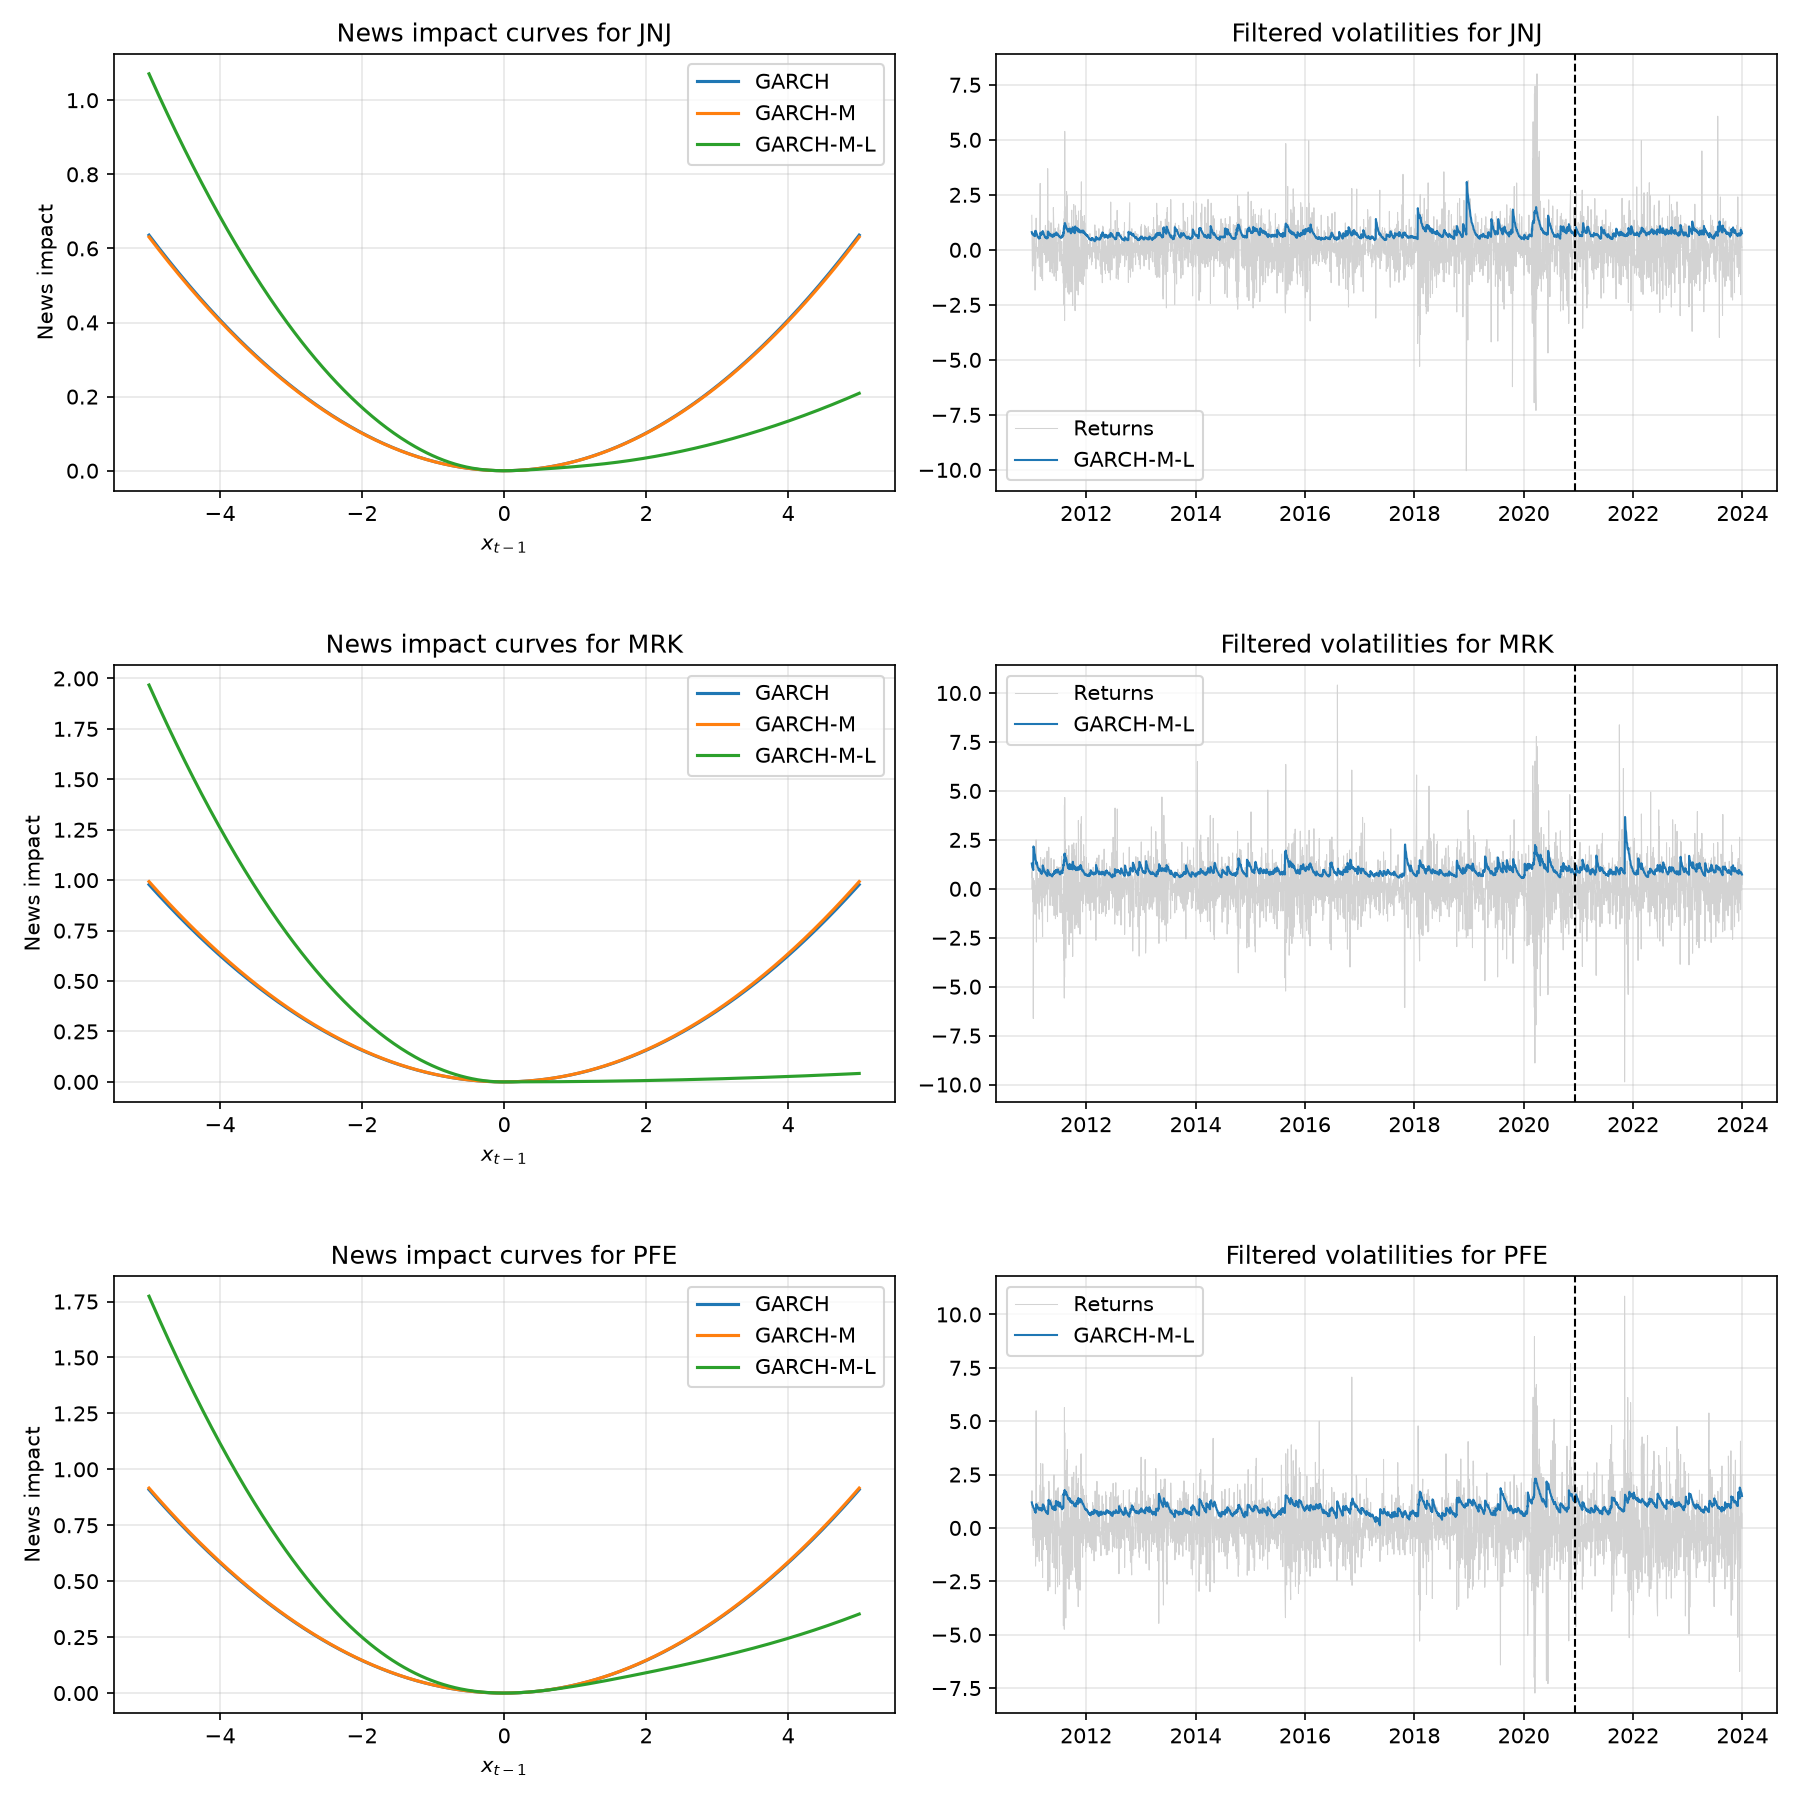
\includegraphics[width=\textwidth]{q5_panels.png}
    \footnotesize
    \begin{minipage}{0.85\textwidth}
    \textbf{Figure 3: News-impact curves and filtered volatilities.} The left panels plot news-impact
    curve $\mathrm{NIC}(x_{t-1}) = (\alpha + \delta \tanh(-\gamma x_{t-1})) x_{t-1}^2$
    for GARCH, GARCH-M, and GARCH-M-L, using each model's estimates from Q4. The right panels plot the observed return
    $x_t$ (grey) and GARCH-M-L filtered volatility $\hat{\sigma}_t$ (blue) over the
    full sample; the dashed line marks January 4, 2021, the end of the in-sample
    window. Stocks: JNJ, MRK, PFE from CRSP daily data, 2011--2023.
    \end{minipage}
    \label{fig:q5_panels}
\end{figure}

The GARCH-M-L news-impact curves are clearly asymmetric for all three stocks, confirming a
leverage effect: negative shocks raise conditional volatility more than positive shocks
of equal size, most strongly for MRK and PFE. GARCH and GARCH-M curves coincide exactly,
since $\lambda$ does not enter the news-impact function. Consistent
with this asymmetry, the filtered volatility for all three stocks rises sharply
following large negative return shocks, most visibly around the COVID-19 onset in
early 2020, while comparable positive shocks produce smaller increases
in filtered volatility. JNJ additionally shows a stock-specific spike in 2019. The filtered
volatility after 2021 remains within a similar range to the in-sample volatility,
suggesting the estimated dynamics generalize reasonably well out-of-sample.

\section*{Question 6}
\begin{table}[H]
    \centering
    \caption{Simulation-based Value-at-Risk estimates}
    \label{tab:q6_var}

    \small
    \setlength{\tabcolsep}{4pt}
    \renewcommand{\arraystretch}{1.15}

    \begin{tabular*}{\textwidth}{
    @{\extracolsep{\fill}}
    ll
    rrrrrrrrr
    }
        \toprule

        Stock & Model
        & \multicolumn{3}{c}{1 step}
        & \multicolumn{3}{c}{5 steps}
        & \multicolumn{3}{c}{20 steps}
        \\

        \cmidrule(lr){3-5}
        \cmidrule(lr){6-8}
        \cmidrule(lr){9-11}

        &
        & \textit{1\%} & \textit{5\%} & \textit{10\%}
        & \textit{1\%} & \textit{5\%} & \textit{10\%}
        & \textit{1\%} & \textit{5\%} & \textit{10\%}
        \\

        \midrule

        PFE & M1
        & -3.78 & -2.24 & -1.62
        & -7.93 & -4.95 & -3.73
        & -14.47 & -9.31 & -6.94
        \\

        PFE & M2
        & -3.76 & -2.19 & -1.58
        & -7.55 & -4.74 & -3.51
        & -13.02 & -8.12 & -5.86
        \\

        PFE & M3
        & -3.82 & -2.28 & -1.63
        & -7.80 & -4.75 & -3.45
        & -13.70 & -8.20 & -5.80
        \\

        \addlinespace[0.8em]

        JNJ & M1
        & -2.41 & -1.42 & -1.02
        & -5.10 & -3.13 & -2.23
        & -10.10 & -5.57 & -3.87
        \\

        JNJ & M2
        & -2.50 & -1.46 & -1.05
        & -5.29 & -3.10 & -2.23
        & -9.29 & -5.60 & -3.89
        \\

        JNJ & M3
        & -2.41 & -1.41 & -1.00
        & -5.18 & -3.00 & -2.16
        & -9.77 & -5.83 & -3.91
        \\

        \addlinespace[0.8em]

        MRK & M1
        & -3.00 & -1.71 & -1.22
        & -5.92 & -3.74 & -2.72
        & -12.02 & -7.15 & -5.08
        \\

        MRK & M2
        & -2.99 & -1.71 & -1.22
        & -6.36 & -3.82 & -2.75
        & -12.05 & -7.39 & -5.29
        \\

        MRK & M3
        & -3.09 & -1.74 & -1.27
        & -6.70 & -4.03 & -2.90
        & -12.18 & -7.53 & -5.45
        \\

        \bottomrule
    \end{tabular*}

    \vspace{0.7em}

    \begin{minipage}{\textwidth}
        \footnotesize
        \textit{Notes:}
        The table reports estimated lower-tail Value-at-Risk (VaR) quantiles for the
        1-, 5-, and 20-day compound holding-period returns at the 1\%, 5\%, and 10\%
        probability levels. M1 denotes the GARCH model, M2 the GARCH-M model, and
        M3 the GARCH-M-L model. Model parameters are estimated using the first
        2,500 observations and are kept fixed while the conditional volatility is
        filtered up to and including January 4, 2021. VaR estimates are based on
        10,000 Monte Carlo simulations and are reported in percentage points.
    \end{minipage}

\end{table}



\end{document}

